\documentclass{article}

\usepackage{cheatsheet}

\renewcommand{\sopName}{ACS}
\renewcommand{\sopVersion}{02-OCT-2016}
\renewcommand{\sopEditor}{(cwe)}


\begin{document}
\fftext%

\maketitle

\notes{%
  \begin{itemize}
    \item \textbf{CAVE:} \hspace{1mm} DD Aortenaneurysma
    \item O$_2$ nur bei SpO$_2$ < 94\% o.\ Dyspnoe
    \item Aspirin auch bei Dauermedikation
    \item Diagnose-to-Balloon < 90 min.
  \end{itemize}
}

\vfill

\drug{Nitrolingual}{%
  \dosierung{1 Hub (\wdh{1} | 3--5 min.)}
  \begin{kontraindikationen}
    \item \textbf{RR} < 110 mmHg
    \item bek. Rechtsherzbelastung bei COPD
    \item diag. Rechtsherzinfarkt
    \item Einnahme PDE-5-Hemmer (Viagra < 24h | Cialis < 36h)
  \end{kontraindikationen}
}

\vfill

\drug{Aspirin}{%
  \dosierung{250 mg i.v.}
  \begin{kontraindikationen}
    \item Asthma / COPD
    \item Ulcus, GI-Blutung, Teerstuhl, Bluterbrechen
  \end{kontraindikationen}
}

\vfill

\drug{Heparin}{%
  \dosierung{60 i.E./kgKG (5000 i.E.) i.v.}
  \begin{kontraindikationen}
    \item Heparin induzierte Thrombozythopenie
    \item Therapierefraktäre Hypertonie
    \item Frische Blutung, GI-Blutung, Teerstuhl
    \item OP, art. Punktion < 7d
    \item bösartiger Tumor
  \end{kontraindikationen}
}

\notes{%
  \begin{center}
    \hspace{-2.5em}
    \rotatebox{90}{\fftext\fontsize{16pt}{16pt}\selectfont\color{myBlue}\hspace{0.4cm}EKG Beispiel}
    \hspace{1em}
    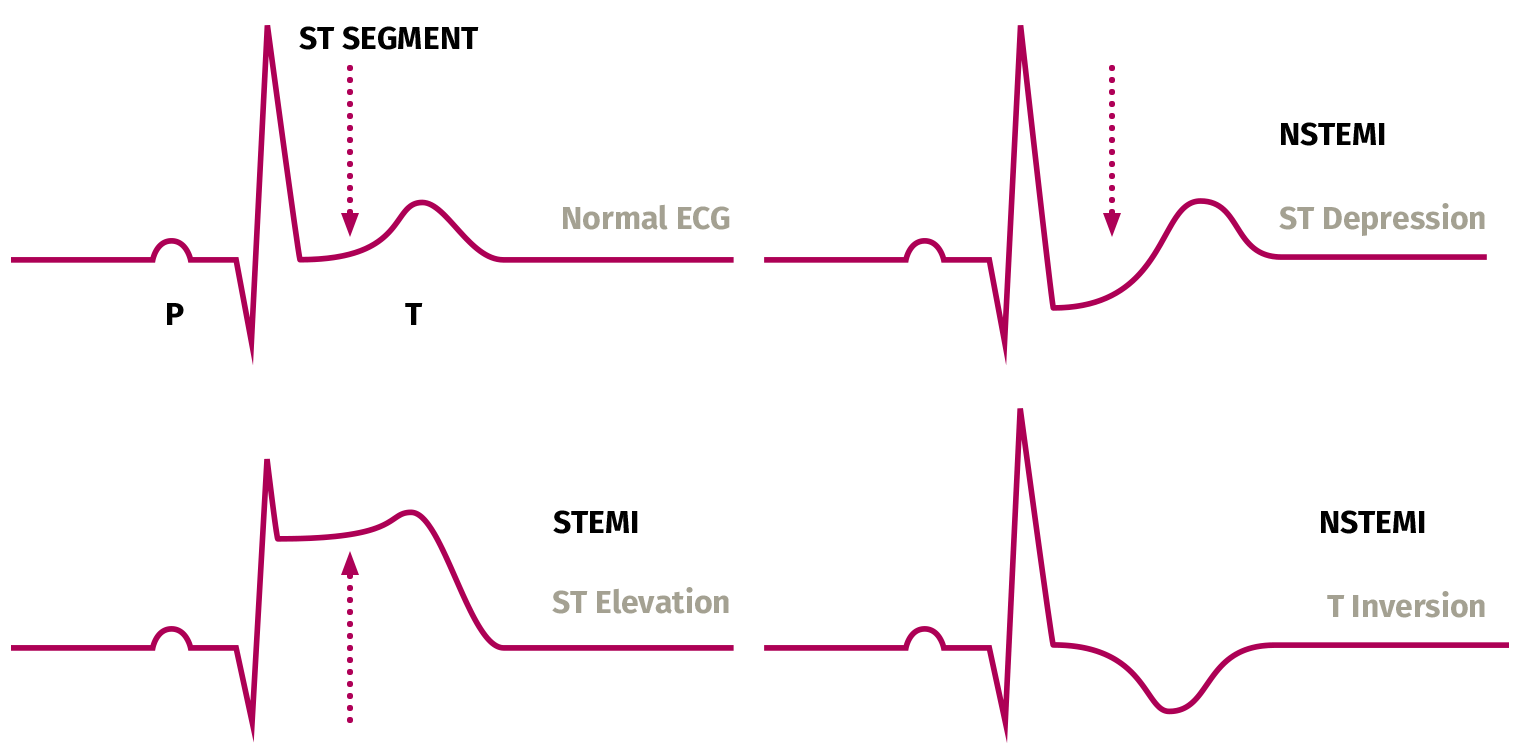
\includegraphics[width=0.75\textwidth]{img/stemi.png}
  \end{center}
}

\vfill

\end{document}
